\chapter{Filesystems}

\section{Introduction}

The filesystem bridges the gap between :
\begin{figure}[h!]
  \begin{center}
    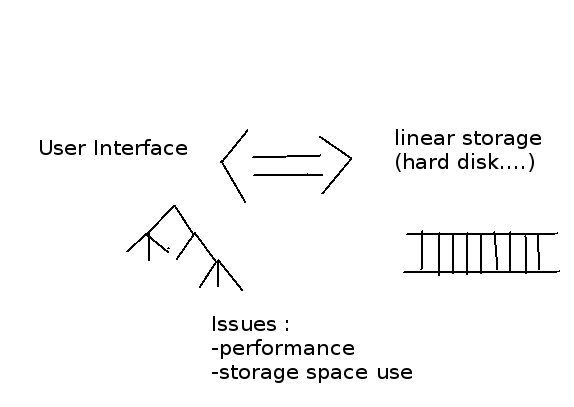
\includegraphics[width=0.6\textwidth]{filesystem.png}
  \end{center}
\end{figure}

\section{User Interface}

Is made of :

\begin{itemize}
  \item files: elementary pieces of information
  \item directories: places which store files and/or directories.
\end{itemize}
  
  One particular directory: root
  \begin{figure}[h!]
  \begin{center}
    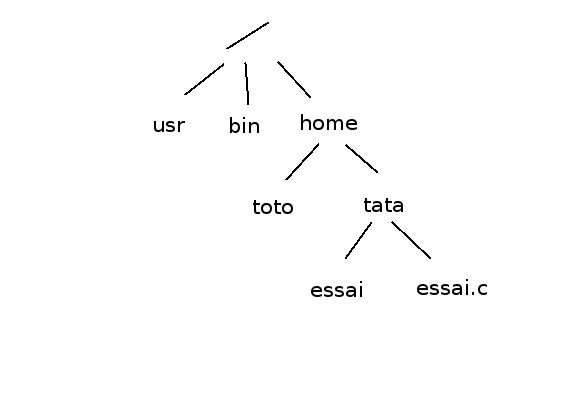
\includegraphics[width=0.5\textwidth]{root.png}
  \end{center}
\end{figure}
  
  Notice : the interface is made in a way that prevents cycles (the FS is a tree).
  
  The user can access to the FS using system calls:

    \begin{center}
      \begin{tabular}{c|c}
         open & opendir \\
         read & readir \\
         write & mkdir \\
         close & closedir \\
         unlink & \\
      \end{tabular}
    \end{center}
This interface is fixe for all existing FS in UNIX.

\section{Organization on the hard disk}

Objectives:

\begin{itemize}
  \item contiguous allocation is better
  \item avoid fragmentation
\end{itemize}

Fact:

\begin{itemize}
  \item accesses to hard disks are performed by blocks, to make worthwhile the fact of paying the latency.
  \item the filesystem can even use larger blocks because accesses (to a given file) are mostly sequential.
  
\end{itemize}

$=>$ there is a risk of increasing internal fragmentation, the block size is a compromise.

\subsection{Linking ---$>$ FAT}

Linked list of blocks, we use a part of the block to link to the next one.

 \begin{figure}[h!]
  \begin{center}
    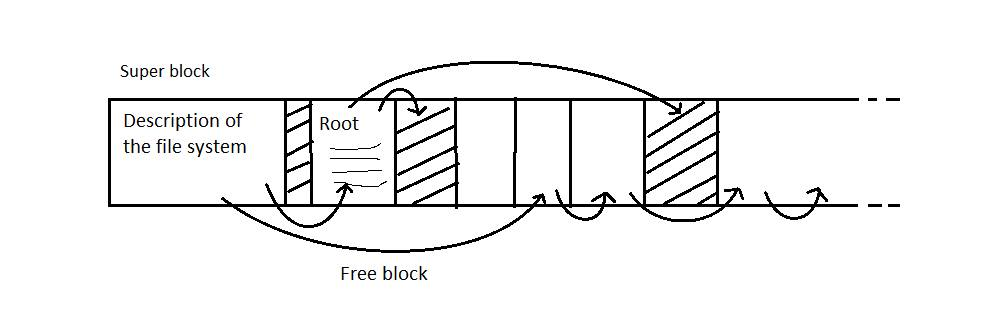
\includegraphics[width=0.8\textwidth]{fat.jpg}
  \end{center}
\end{figure}

Directories are special files which contain a sequence of couples : filename \& number of first block (of the file).

Files and Directories start with a meta data block which contains:
\begin{itemize}
  \item type of file
  \item permissions
  \item size
  \item access times
  \item ...
\end{itemize}

Not efficient: random accesses to files are not efficient because they require the reading of all the blocks.

Idea to solve the issue, place the linking information elsewhere.

Normal use:
\begin{itemize}
  \item opening: not efficient (one has to read all the directories on the path) but performed once. $--->$ number block of metadata of the file.
  \item read: ok, jump from block to block.
  \item lseek, open(append mode) :   not efficient.
\end{itemize}

$=>$ File Allocation Table (FAT)

Still, there are several accesses when randomly accessing to a large file.

$=>$ usually the whole table is cached into memory.

\begin{figure}[h!]
  \begin{center}
    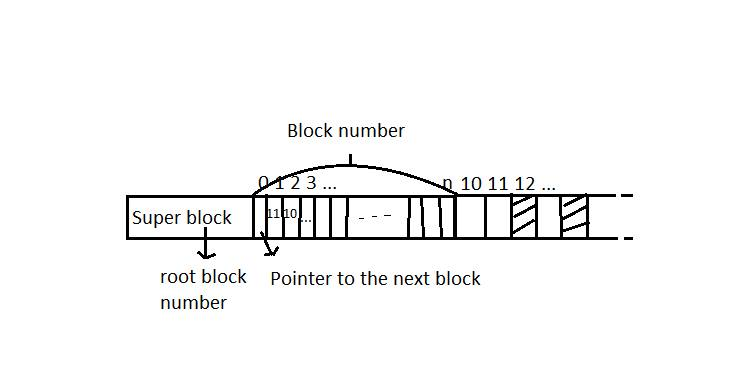
\includegraphics[width=0.8\textwidth]{fat_2.jpg}
  \end{center}
\end{figure}

\subsection{Inodes and allocation tables}

The inode combines:
\begin{itemize}
  \item meta data related to a file
  \item index of data blocks of the file
\end{itemize}

Stored on a single block, the size of the index is limited, ex: 12 entries in inodes in ext2.

\begin{figure}[h!]
  \begin{center}
    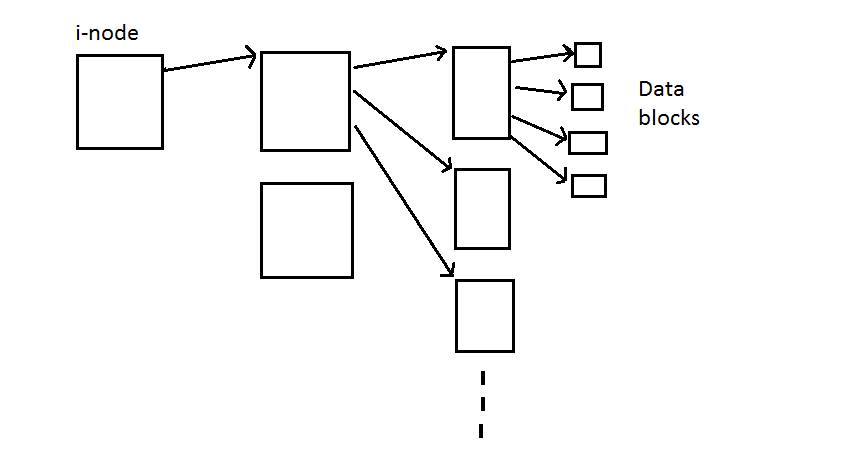
\includegraphics[width=0.5\textwidth]{inode.jpg}
  \end{center}
\end{figure}

$--->$ An inode also contain indirect links:
\begin{itemize}
  \item one single indirection link: points to a block which contains pointers to data blocks.

  \item one double indirection link: points to a block which contains pointers to data blocks which contains pointers to data blocks.
  \item one triple indirection link : points to ....
  
\end{itemize}

The assesses:
\begin{itemize}
  \item are very efficient for small files (direct links in the inode)
  \item are less efficient for large files (up to three indirect links) but it is bounded by a constant factor.
\end{itemize}

Overall organization:

 \begin{figure}[h!]
  \begin{center}
    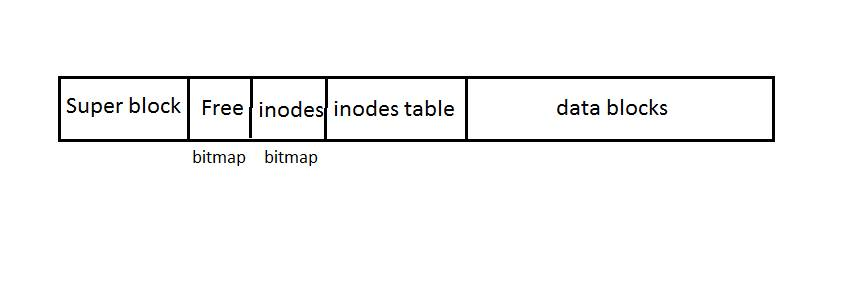
\includegraphics[width=0.8\textwidth]{inode_2.jpg}
  \end{center}
\end{figure}

\section{Fragmentation}

Different from fragmentation in the memory allocator: here it is related to the fact that data blocks of a file are not necessarily contiguous.

 \begin{figure}[h!]
  \begin{center}
    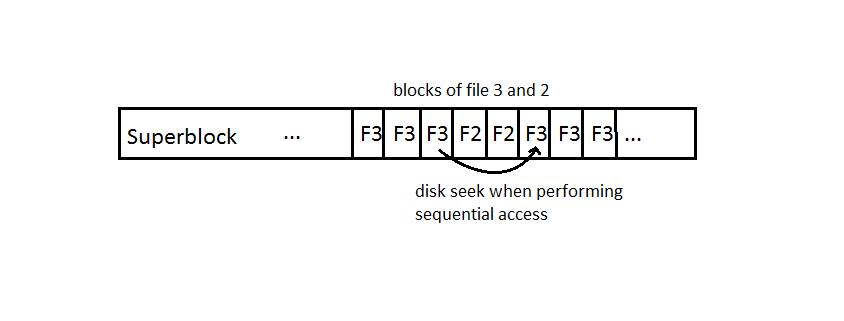
\includegraphics[width=0.8\textwidth]{fragmentation.jpg}
  \end{center}
\end{figure}

$=>$ defragmentation tools: exchange blocks all accross the disk.

$=>$ not efficient

Another idea is to avoid fragmentation as much as possible within the FS.

Ideas: (Fast File System)
\begin{itemize}
  \item  try to keep small files close to each other
  \item try to divide the whole storage space into several local groups.
  \item spread large files into different groups by dividing them into large chunks.
\end{itemize}

Thus a compromise:
\begin{itemize}
  \item large chunks to limit seeks
  \item file divided into chunks to keep flexibility and avoid eventual fragmentation
\end{itemize}
\begin{figure}[h!]
  \begin{center}
    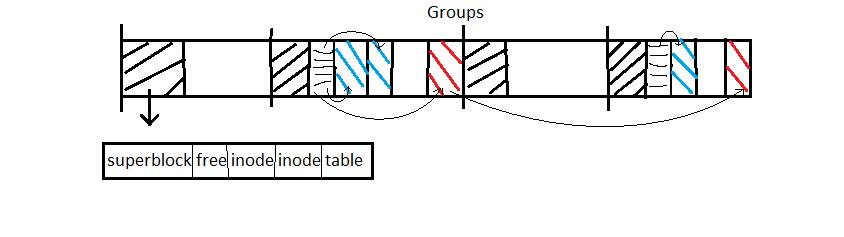
\includegraphics[width=\textwidth]{fragmentation_2.jpg}
  \end{center}
\end{figure}
These optimization are mainly common sense but they work very well in practice.

\section{Filesystem updates \& failures}

Ex: to append a block to a file (ex: /var/log/syslog)
\vspace{1cm}
\begin{figure}[h!]
  \begin{center}
    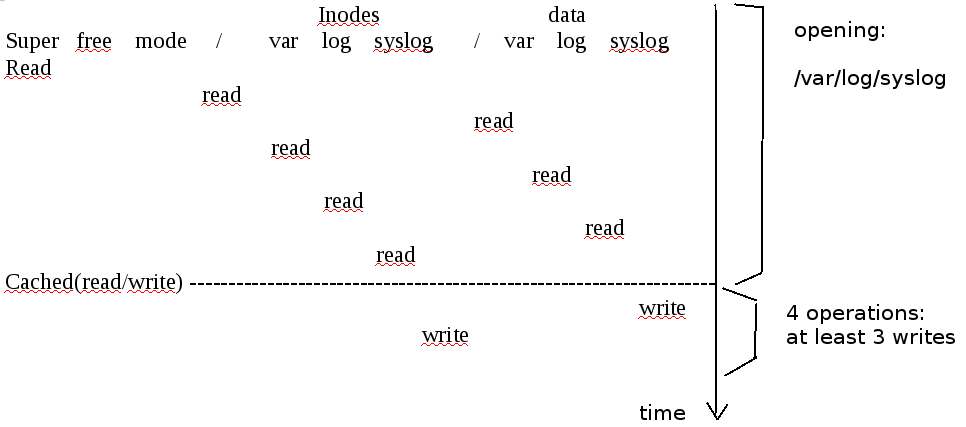
\includegraphics[width=0.8\textwidth]{fs_updates_failures.png}
  \end{center}
\end{figure}


An access is costly because of FS structure updates

$=>$ the FS cache accesses to memory:
\begin{itemize}
  \item as many as possible for reads
  \item during some time for writes (5-30s)
\end{itemize}
compromise between efficiency and risk of loosing data in the case of power failure.

If there is a power loss, cached writes might be:

\begin{itemize}
  \item completely in memory
  \item poartially onto disk:
    \begin{itemize}
      \item corrupted FS
      \item incorrect data blocks
    \end{itemize}
\end{itemize}
